
\documentclass[11pt,twocolumn,a4paper]{article}



\usepackage[hmargin={1.35cm,1.35cm},vmargin={2.0cm,3.0cm},footskip=0.75cm,headsep=0.25cm]{geometry}


%\usepackage[
%backend=biber,
%style=ieee,
%sorting=none
%]{biblatex}
%\addbibresource{muscleBib.bib}

\usepackage{amsmath, amssymb}
\usepackage{commath}
\usepackage{graphicx}
\usepackage{fancyhdr}
\usepackage{authblk}
\usepackage{xcolor}
\usepackage{hyperref}
\usepackage[switch,columnwise]{lineno} 
\usepackage{multicol}


%
% 1. User defined commands.
%    Here you can define commands (defined in the first braces)
%    that are replaced with the text in the second pair of braces
%    when you compile the document.
%
%    I use these for 3 purposes:
%    a. Defining mathematical notation
%    b. Defining abbreviations
%    c. *Defining specific numerical results
%
%    I do this so that I only have to check the document in 
%    one location to see if I got these things correct. The 
%    alternative is that you manually look through the document
%    (spell check is not enough: you can have spelling errors in 
%    your abbreviations). This is error prone and frustrating so 
%    I automate this using \newcommand statements.
%
%    *I will even set up my matlab scripts to write these commands
%     to file so that when my simulations change I get an 
%     automatically generated set of 'newcommand' statements
%     that I just have to paste in place. Because this is tedious
%     I try to avoid reporting numerical results in text:
%     figures and tables are better spots. But sometimes this
%     is unavoidable.
%

%1a. Standard mathematical notation: 
%    example muscle modelling notation
\newcommand{\mpss}{\mathrm{m}/\mathrm{s}^2}
\newcommand{\cOne}{\mathcal{C}^1}
\newcommand{\cTwo}{\mathcal{C}^2}

\newcommand{\fiso}{f_{\mathrm{o}}^{\;\!\mathrm{M}}}

\newcommand{\kx}{k^{\;\!\mathrm{X}}}
\newcommand{\kxiso}{k_{\mathrm{o}}^{\;\!\mathrm{X}}}
\newcommand{\ktNiso}{\tilde{k}^{\mathrm{T}}_{\mathrm{o}}}
\newcommand{\kxisoNorm}{\tilde{k}_{\mathrm{o}}^{\;\!\mathrm{X}}}

\newcommand{\dxiso}{\beta_{\mathrm{o}}^{\;\!\mathrm{X}}}
\newcommand{\dxisoNorm}{\tilde{\beta}_{\mathrm{o}}^{\;\!\mathrm{X}}}


\newcommand{\ftC}{\mathbf{f^{\;\!\mathrm{T}}}}
\newcommand{\flC}{\mathbf{f^{\;\!\mathrm{L}}}}
\newcommand{\fvC}{\mathbf{f^{\:\!\mathrm{V}}}}
\newcommand{\fpeC}{\mathbf{f^{\;\!\mathrm{PE}}}}

\newcommand{\lopt}{\ell_{\mathrm{o}}^{\;\!\mathrm{M}}}
\newcommand{\lm}{\ell^{\;\!\mathrm{M}}}
\newcommand{\lmt}{\ell^{\;\!\mathrm{MT}}}
\newcommand{\lt}{\ell^{\;\!\mathrm{T}}}

\newcommand{\et}{e^{\;\!\mathrm{T}}_{\mathrm{o}}}
\newcommand{\etToe}{e^{\;\!\mathrm{T}}_{\mathrm{toe}}}
\newcommand{\lsk}{\ell_{\mathrm{s}}^{\;\!\mathrm{T}}}


\newcommand{\vmt}{v^{\;\!\mathrm{MT}}}
\newcommand{\vm}{v^{\;\!\mathrm{M}}}
\newcommand{\vt}{v^{\mathrm{T}}}
\newcommand{\vtN}{\tilde{v}^{\;\!\mathrm{T}}}
\newcommand{\vmax}{v_{\mathrm{max}}^{\;\!\mathrm{M}}}

\newcommand{\pen}{\alpha}
\newcommand{\penopt}{\alpha_\mathrm{o}}
\newcommand{\act}{a}
\newcommand{\ex}{u}
\newcommand{\actTime}{\tau_{\mathrm{A}}}
\newcommand{\decayTime}{\tau_{\mathrm{D}}}

\newcommand{\dTendonConstA}{V}
\newcommand{\dTendonConstB}{U}

%1b. Defining abbreviations: 
%    example abbreviations
\newcommand{\ce}{CE}
\newcommand{\xe}{XE}
\newcommand{\mtu}{MTU}
\newcommand{\vexat}{VEXAT}
\newcommand{\caTwoPlus}{\mathrm{Ca}^{\mathrm{2+}}}


%1c. Defining specific numerical results
%
\newcommand{\titinPradoLow}{24\%}
\newcommand{\titinPradoHigh}{57\%}

\newcommand{\ecmPradoLow}{43\%}
\newcommand{\ecmPradoHigh}{76\%}
\newcommand{\ecmPrado}{56\%}

\newcommand{\EcmTitinProp}{\mathrm{P}}
\newcommand{\EcmTitinPropNum}{0.56}
\newcommand{\EcmPercent}{56}
\newcommand{\TitinPercent}{44}

\newcommand{\tendonDampingFactor}{0.057}

\newcommand{\kmFitToKirschFigThree}{3.53 N/mm}
\newcommand{\ktFitToKirschFigThree}{16.9 N/mm}
\newcommand{\kceATFitToKirschFigThree}{4.46 N/mm}
\newcommand{\kceFitToKirschFigThree}{4.46 N/mm}
\newcommand{\kmNormFitToKirschFigThree}{7.04}



%%%%%%%%%%%%%%%%%%%%%%%%%%%%%%%%%%%%%%%%%%%%%%%%%%%%%%%%%%%%%%%%%%%%%%%%%%%%%%%%%%%%%%%%%%%%%%%%%%%%
%%  Macros for use in text
%%%%%%%%%%%%%%%%%%%%%%%%%%%%%%%%%%%%%%%%%%%%%%%%%%%%%%%%%%%%%%%%%%%%%%%%%%%%%%%%%%%%%%%%%%%%%%%%%%%%
\newcommand{\unit}[1]{$\left[\mathrm{#1}\right]$}


% Include other packages here, before hyperref.

% If you comment hyperref and then uncomment it, you should delete
% egpaper.aux before re-running latex.  (Or just hit 'q' on the first latex
% run, let it finish, and you should be clear).
%\usepackage[pagebackref=true,breaklinks=true,a4paper=true,colorlinks=false,bookmarks=false]{hyperref}
%\usepackage{lineno}
%\pagewiselinenumbers

\renewcommand\Affilfont{\fontsize{9}{10.8}\itshape}


\lhead{} \chead{An example \LaTeX{} document} \rhead{}
\lfoot{} \cfoot{\today, Quick Brown Fox, p. \thepage} \rfoot{}

\title{An example \LaTeX{} document}

\author[1,2]{Quick Brown Fox}
\author[3]{Lazy Dog}
\affil[1]{Fox Research, Baden-W\"{u}rttemberg, Germany}
\affil[3]{Department of Dackl, Badger University, Hessen, Germany}
\affil[*]{\tt\small fantastic.fox@uni-fox.de}


\begin{document}

\linenumbers


\maketitle


\abstract{ 



The quick brown fox jumped over the lazy dog. 

}

\section{Introduction: citing literature}

%Use this label to refer to the introduction by typing 'Sec. \ref{sec:intro}'
\label{sec:intro}

If you're interested in using \LaTeX{} I recommend that you get a text editor that has syntax highlighting. I've used the following tools:
\begin{itemize}
    \item Notepad++ (windows)\\ \url{https://notepad-plus-plus.org/}
    \item Sublime text (linux)\\ \url{https://www.sublimetext.com/}
    \item Overleaf (online)\\ \url{https://www.overleaf.com/}
    \item vi/vim (linux, comes pre-installed)
\end{itemize}    
I also recommend you pick a tool with a good spell check, ideally one that is aware of \LaTeX{} syntax. Now that you have one of these tools installed, open main.tex and muscleBib.bib and have a look. The file main.tex has comments in it (\# is the comment character) to help you through the file. While this file will give you an introduction, for more details I recommend a good book such as the one I used when starting: A guide to \LaTeX{} by Helmut Kopka and Patrick Daly.

Citing a single reference is done using the $\backslash$cite command as in \cite{Trumbower2009PostureStiffness}. To cite multiple authors simply add the other citation key separated by ',' to the arguments given between the '\{' '\}'. For example \cite{KayaHiguchi2013MyosinStiffness, AbbottAubert1952:RampStretch}. The entries for each cite command need to be stored in a bib file (see the attached muscleBib.bib file). The file muscleBib.bib is just a text file, so you should open it up in the text editor and look at it along with this file.

These entries were manually put into the bib file. The entries can be found in a few different ways:
\begin{enumerate}
\item Google scholar\\ \url{https://scholar.google.com/}
\begin{enumerate}
    \item Find the paper
    \item Click 'cite'
    \item At the bottom click 'BibTex'. After that the entry BibTex should be displayed.
    \item Note: this entry is often missing the doi, and sometimes has errors
\end{enumerate}    
\item The publisher's page often has an option to download the BibTex 
\item A paper management system (like Mendeley) will provide this text
\end{enumerate}    

To compile the document and the bibliography:

\begin{figure*}[t]
    \centering
    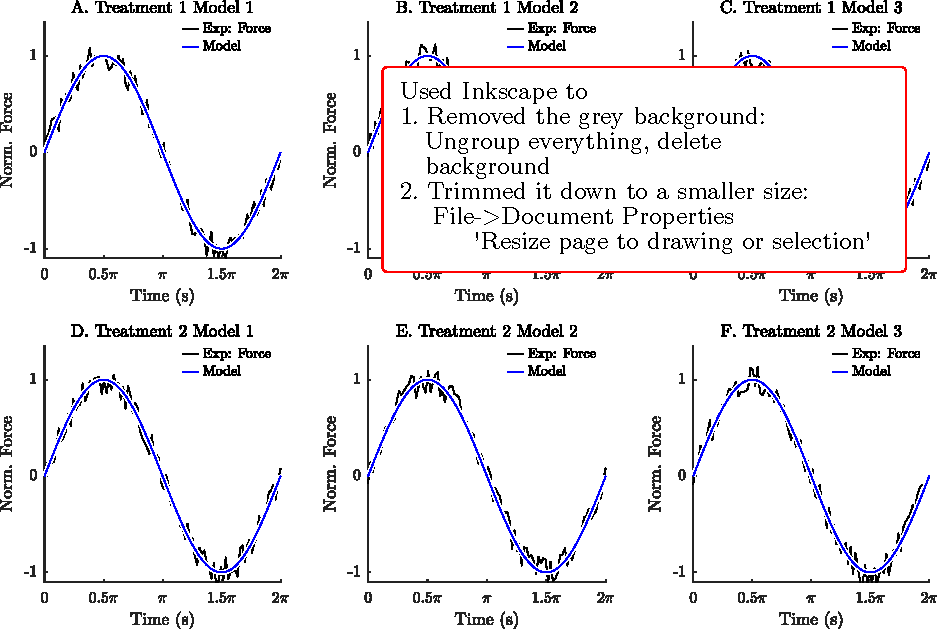
\includegraphics{figures/fig_exampleSingleColumnPlot.pdf}
    \caption{Since the figure is correctly sized already, no extra options are needed: the figure and all of its fonts will appear exactly at the correct size. However, the options 'width=$\backslash$textwidth' and 'keepaspectratio=true' are often used to make the figure fit the full width of the text area (which will make the fonts bigger in this case). Note that the \textbf{figure*} environment is used here rather than \textbf{figure}: the \textbf{*} is needed to add a full-width figure to a 2 column document. Finally, one of the most frustrating things to a beginner is getting \LaTeX{} to put the figure where you want it to appear. The easiest way to do this is to move this command either earlier or later in the text, recompile, and then see if you like the result. The next approach is to suggest a location using the optional figures commands: $\backslash$begin\{figure*\}[h] for here, [!h] for here (more strongly), [t] for top, and [b] for bottom.
    \label{fig:model}}
\end{figure*}

\begin{enumerate}
\item Make sure you have a working version of \LaTeX{} installed on your system.    
\item Open a terminal window in the same folder as the *.tex file
\item Enter the following commands
\begin{enumerate}
    \item pdflatex main.tex
    \item bibtex main.aux
    \item pdflatex main.tex    
\end{enumerate}    
In the first command the pdf is generated without references (these will appear as `?' at this point). However, the names of the needed references are stored in the 'main.aux' file. Calling 'bibtex main.aux' will generate a formatted bibliography stored in the 'main.bbl' file. Finally calling pdflatex main.tex a final time will put these references into the pdf document. If you use overleaf these multiple calls are hidden from you.
\item If the document doesn't compile, don't panic:
\begin{enumerate}
    \item Read the error message in the window. It usually tells you where in the document the problem is located.
    \item Try fixing the error, and if you can't, look online: there's a lot of good help online if you can describe the problem.
    \item You may need to delete the 'main.aux' file. 
    \item Then try, try again.
\end{enumerate}
\end{enumerate}    




\section{Methods: cross-references + user-defined commands + figure + equation}

\label{sec:model}


Now that you've read Sec. \ref{sec:intro} (cross-reference to the introduction) we can move onto more interesting things such as cross-referencing a figure (Fig. \ref{fig:model}), a table (see Table \ref{tbl:archprop} in Appendix \ref{sec:catSoleusProperties}), and even inserting an equation such as Eqn. \ref{eqn:xbridgeStiffness}. 
This cross-referencing is all done using the same $\backslash$label\{\} and $\backslash$ref\{\} commands. Note, if you look at this text you'll see that $\backslash$ is typeset using a command because it is a special character.




Speaking of commands, all of the newcommand statements in the preamble can be used in the text, for example: $\fiso$, and $\lopt$. These can also be used in equations
\begin{equation}
\kxiso = \kxisoNorm \dfrac{\fiso}{\lopt},  \label{eqn:xbridgeStiffness}
\end{equation}
and in tables as is shown in Table \ref{tbl:archprop} in Appendix \ref{sec:catSoleusProperties}.


\section{Homework}

\begin{enumerate}
\item Convert this document to a single-column document by changing 'twocolumn' to 'onecolumn' in the statement that appears on the first line.
\item  Use the textcolor \textcolor{blue}{command} to change the color of this word to red.
\item Be aware that BibTex is pretty simple. If you want to have a bibliography with the doi then you'll need to use something like biber. The statements needed to use biber appear in this document on lines 9-14 (currently commented out) and the $\backslash$printbibliography statement below. You can try using biber:
\begin{enumerate}
    \item Check if it's installed by entering 'which biber' (for linux) into a command terminal. If you're working on windows search online for a suggestion.
    \item Uncomment the statements on lines 9-14
    \item Comment the 3 lines immediately after the acknowledgement section (lines 280-283)
    \item Uncomment the $\backslash$printbibliography
    \item Delete main.aux and main.bbl
    \item In a terminal:
    \begin{enumerate}
        \item pdflatex main.tex
        \item biber main
        \item pdflatex main.tex
    \end{enumerate}
    \item If it worked you should see hyperlinked doi numbers for most entries in the references section.
\end{enumerate}

\end{enumerate}

\section*{Acknowledgements}

By adding a * to the section command ($\backslash$section*\{\}) the number in front of the section title is removed. This is perfect for Acknowledgment statements.

{\small
\bibliographystyle{ieeetr}
\bibliography{muscleBib}

%\printbibliography


\newpage
\appendix



\section{An example appendix section}
\label{sec:catSoleusProperties}


Just by adding the command $\backslash$appendix (which appears here after the $\backslash$bibliography\{muscleBib\} statement) the section numbering will switch to using alphabetical characters. 
For your final example, you can find an example of a typesetting a simple table here in Table \ref{tbl:archprop}. 
The tabular environment is used to make the table, while the table environment is used to turn it into a float: that is something that has a caption and can be moved around.

\begin{table}
\caption{Cat soleus \mtu{} properties used in this work. \label{tbl:archprop}}
\begin{center}
\begin{tabular}{l l | l | l} 
Parameter                 & Symbol            & Value            & Source \\
\hline Optimal \ce length & $\lopt$           & 42.9 mm          & \cite{HerzogLeonard2002ForceEnhancement} \\
Pennation angle           & $\pen$            & $7^\circ$        & \cite{Sacks1982CatLegMuscleArch} \\
Max. iso. force           & $\fiso$           & 21.4 N           & \cite{HerzogLeonard2002ForceEnhancement} \\
Max. shortening vel.      & $\vmax$           & 4.5 $\lopt/s$    & \cite{Scott1996MechanicsI} \\
Tendon slack length       & $\lsk$            & 30.5 mm          & \cite{Scott1995CatTendonModel} \& \cite{HerzogLeonard2002ForceEnhancement} \\
Tendon stiffness          & $\ktNiso$         & 30 $\frac{\fiso}{\lsk}$            & \cite{Scott1995CatTendonModel} \\
Tendon damping            & $\dTendonConstB$  & $\tendonDampingFactor \frac{1}{s}$ & \cite{Netti1996TendonLigament}   \\ 
ECM fraction              & $\EcmTitinProp$   & \ecmPrado{}                        & \cite{Prado2005ECMandTitin}
\end{tabular}
\end{center}
\end{table}


\end{document}

